\chapter{Introduction}

\textbf{Welcome to CIS 2520!}

A data structures course is often the first course in a series of courses on software design.  
During this class we will examine a variety of abstract data types and how they can be used to improve the quality of the software you develop. This e-text contains all the notes provided as part of the course website as well as more detailed material for in-depth study.  
 
The examples will be given in pseudo code that could be used as the outline for a program in nearly any programming language, or in c.   The pseudocode format is as follows:  

\begin{itemize}
\item function and procedures are defined with a name that begins with a lower case 
\item parameters are included as types only 
\item if there is a return value,   it appears at the end of the function definition after a colon
\item no ending punctuation is used for lines
\item indentation is used rather than parentheses  
\end{itemize} 
For example a pseudocode function could be defined as :    

\begin{lstlisting}
calculateComplicateValue(int, String): int
\end{lstlisting}
 If the same function were actually written in a C header file it would look something like this:  
 \begin{lstlisting}
 int calculateComplicateValue(int intVal, char * stringVal);
 \end{lstlisting} 
\section{Why Software Design}

Most software is not developed by a single person and most of it takes months or even years to complete and test.   Most software development involves multiple people who subdivide the problem into chunks and then collaborate to make the entire program work.
 
The process of identifying suitable chunks is the essence of software engineering.   When the chunks are defined so that a single chunk can be reused in more than one software project, the company benefits because it only pays once for the development of something than can be used more than once.  Good software engineering   practices save time (on the part of the developer) and money (on the part of the employer or funding organization).


In future courses, you will spend time learning about a variety of formal approaches to software development.    Each formal approach represents one way to try to meet the objectives of modularity, maintainability, reuse, low coupling, high cohesion when creating software with medium-large teams. The effectiveness of each formal approach depends on the type of software being developed, on the development environment and context, and on the personalities of the development team.


\section{Software Development- CIS 2520 Style}

Clean, crisp coding habits are developed over time, not learned all at once.   And, like any good (or bad) habit, if you don’t practice, you’ll lose the habit.   You are expected to follow good coding practices for all of your homework in this class.     Consistency is the key to writing readable code.   For all work for 2520, you are expected to follow the following minimum set of conventions.

\begin{itemize}

\item Use a consistent naming convention for all variable names.  Variable names must be meaningful with single-character names used only for counters.
\item The names for types (including abstract data types) must be obviously different from the names for variables.  For example, you could capitalize the first letter of the names of a type.
\item Use spaces for indentation- do not use tabs
\item Use .h files to declare functions and types and put implementation in .c files.  You may, or may not, need a .h file for the file containing main.   Use include-guards in your .h files.
\item Organize your .h files and .c files so that functions are in the same order in both files.  Use blank lines to create groups of code.   
\item Doxygen style comments go in the .h file for every function (as a minimum)  
\item Every source code  or .h file begins with a doxygen comment  that indicates author, purpose of code, and last modification date.
\item Compile your code with -Wall and -g flags.  You may use -ansi, -std=c99 or -std=c11
\end{itemize}


You must submit modular code for your homework solutions.  This means you must break programs into separate files.   
\begin{itemize}
\item Use makefiles to automate the build process so that you can divide your code into as many modules as necessary.    
\item Each file in your project should contain a single module that goes together in some way (i.e. a module for reading in files,  a module for calculating things,  a module for list operations).
\item Your programs must be organized in a file structure that contains src/  bin/ include/  assets/  and docs/  folders and your makefile must make use of that file structure.   src/ is for source code,  include/ is for .h files,   docs/ is for doxygen documentation,  and assets is for testing files, data files, etc.   The README goes in the root folder of an assignment, not in the sub folders.
\item The README file should be based on the template shown at the end of this chapter.  Read assignment specifications carefully as there may be additional information  expected in assignment-specific README files.
\end{itemize}

\section{Test driven development }

 It is not enough to simply have a program that runs,   it must run properly and produce correct results for all allowable inputs.  One way to do that is to set up the testing program as the first thing you do, and then to test early and to test often.   
 
 Instead of writing the entire solution to your homework, create a skeleton that that is just the framework of your program but no functionality.  The skeleton should have all the files, all the functions  definitions,  all the structures and types, but none of the actual functionality.  The values returned by functions and any actual data processing is completely hard coded.    This is called writing a \textbf{stub} for a function.  
When you have created a complete skeleton for your program, you can then add functionality to one function or procedure at a time and test just that function.
 
Use a driver or test harness to test your code modules.  Write the test harness as a series of function calls in main, using hard coded data for which you know the return value.  Add checks and comparisons to determine if value returned by your function is the expected value.  Once your software can pass all of the tests in your test harness, then it is time to write a new 'main' that is the actual application.
 
Create test data that cover all the different types of possible data.   Test for edge cases (zero or null values,   really big values, too many values, etc).   Test each function with  values having different attributes so that you can show you have thoroughly tested the different parts of your software.

For example,  below you can find  the skeleton code for a singly linked list of string data.  You have likely worked with linked lists in a previous course.  The code given contains no functionality, but it will compile and run with a test harness.    Note:  This skeleton code should not be your starting point for the first lab as it does not meet the requirements for the first lab.   The skeleton code also gives you an example of doxygen-styled comments, which are required for this course and of how to use include guards in your .h file.


The .h file contains the function prototypes and the struct definitions and  the comments for each function.
\begin{lstlisting}
/**
 * @file linkedList.h
 * @author Judi McCuaig
 * @date January 2017
 * @brief API for a singly linked list
 */
#ifndef _JRM_LLIST
#define _JRM_LLIST
struct listNode {
    char * nodeValue;
    struct listNode * next;
};
typedef struct listNode node;

/** Creates a list and returns a pointer
*@return pointer to the list head
**/
node * createList ();
/** Destroys the list and frees all the allocated memory
*@param pointer to the head of the list
**/
void destroyList(node * head);
/** Adds an element to the head of the list
*@param pointer to the head of the list
*@param pointer to the string that will be stored in the list
**/
void addFront (node * head, char * data);
/** Removes a specific element from the list and frees the memory for that element
*@return 0 if the removal is successful, -1 on error
*@param pointer to the head of the list
*@param pointer to the string that will be removed from the list
**/
int removeFromList(node * head, char * data);
/** Prints the list in head-to-tail order
*@param pointer to the head of the list
**/
void printList(node * head);
/** Frees the memory allocated for a list node
*@param pointer to the node to be freed
**/
void freeElement (node * element);
/** Creates a list node with the data provided in the parameter
*@return pointer to the new node
*@param pointer to the data to be stored in the node
**/
node * initElement(char * data);

#endif
\end{lstlisting}

\clearpage
The source code (.c) file contains the implementation for the functions.
\begin{lstlisting}
/**
 * @file linkedList.c
 * @author Judi McCuaig
 * @date January 2017
 * @brief skeleton code for a singly linked list
 */
#include "linkedList.h"

node * createList ()
{
       return (NULL);
}

void destroyList(node * head)
{    
}

void addFront (node * head, char * data)
{    
}


int removeFromList(node * head, char * data)
{
   return(0); 
}


void printList(node * head)
{
    printf("\n");
}


void freeElement(node * element)
{
}

node * initElement(char * data)
{
}
\end{lstlisting}

\section{Extending Activities}

\begin{itemize}

\item The internet has many high quality resources about software engineering and software design.  Build yourself a list of resources for information.  Look for podcasts, videos, websites, or newsgroups that can help you arrive at definitions for each of the following:   Modularity,   Reuse, Maintainability,   Coupling,   Cohesion.     You may use Wikipedia, but try to find other resources as well.



\item There are many different processes for developing software.  A common (and old) process is called the Waterfall cycle and involves rigidly dividing the process into definition, design, development and testing segments.  Each segment is completed before the next segment is started.  Other processes are more fluid, moving between design and development as new requirements are noted.
 It is very difficult to use a formal software development process as part of coursework because most of the design process is done for you when the assignment specification is done.   Still, it is possible to use portions of specific approaches.   The lab activities for 2520 are based on a modified Test-Driven development cycle.    Use internet resources to inform yourself about Test-Driven development.  Make list of the changes you will need to make to your own development habits in order to be successful in a test-driven process.
\end{itemize}

\chapter{Abstraction}

\section{Introduction}
While computer hardware has changed significantly over the past several decades, the way in which we communicate with computers has not changed very much at all. The basic instructions and building blocks used in a computer program are the same now as they were when computers were constructed from mechanical parts.
At the machine level, a program is a set of instructions composed of arithmetic and logic, and the data used and the instructions of the program are all represented as binary numbers. Most programmers rarely, if ever, interact directly with the binary machine code when creating computer programs. Instead a programmer uses a higher level language, an abstraction, that provides single instructions that represent several machine code steps.
For example, in machine code, the instruction to add two numbers might look something like this:

00001001 0000000001100011 000000000110010

where the first number represents the instruction for add, and the second number is the memory location of one value to be added and the third number is the memory location of the second value to be added. This example code does not include putting the result of the addition anywhere useful for the programmer- that is a second step.
Abstracted programming languages greatly improved the productivity and reliability of the programs written. Such languages are often called 'high level' languages. C, Pascal, Cobol, LISP, and Fortran are among the first high level languages developed. Each of these languages was specialized somewhat to create usable abstractions for operations that were common to a particular class of computer programs. Cobol has specialized operations for business and was created so that even non-programmers could understand the code. Fortran is specialized for mathematics, and LISP is specialized for artificial intelligence programming.
In more recent years, even higher level languages have been abstracted from the early languages



\section{Real World Abstraction}
Abstraction is a tool that we use to navigate the world around us. A map is an example of an abstraction. A map contains information about a real space, but it only contains the information that is relevant to moving around in that space. Maps do not contain ALL the details about a space because that would make the map unreadable.

An abstraction is a representation of something that shows only the details that are essential for the task at hand, and ignores the other details. Think again about the map example. A topographical map has different details than a street map. A map that outlines points of interest for a nature walk would have different details than a map constructed for a geological survey.

Abstraction is used to make devices usable in situations where it is unnecessary to understand all the details in order to use something. The modern car is usable by persons who have little or no mechanical aptitude. The details that the driver sees are relevant for safe driving, and all the details about how the car operates have been hidden from the driver.

The utility supply to your house is an abstracted interface. You can use electrical power in your house without needing any details about how that power is generated, or how your house is wired. You don't even need to understand how electricity works.
A good abstraction is one that simplifies the use of something, but that still permits use in many general situations. Sometimes abstraction is unnecessary.


Consider the kitchen can opener. Many different kinds of can openers can be purchased, with a widely varying level of abstraction. Each higher level abstraction hides a few more details about how the can opener works. All can openers eventually open the can, the difference is in the amount of effort and understanding required of the operator.

\begin{figure}[H]
\centering
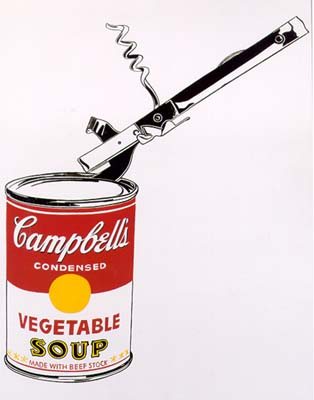
\includegraphics[width=0.3\textwidth]{pictures/Campbell_s_Soup_with_Can_Opener.jpg}
\label{fig:canOpener1}
\end{figure}

This example makes it very clear that the can is opened by wiggling a sharp knife up and down through the metal.

\begin{figure}[H]
\centering
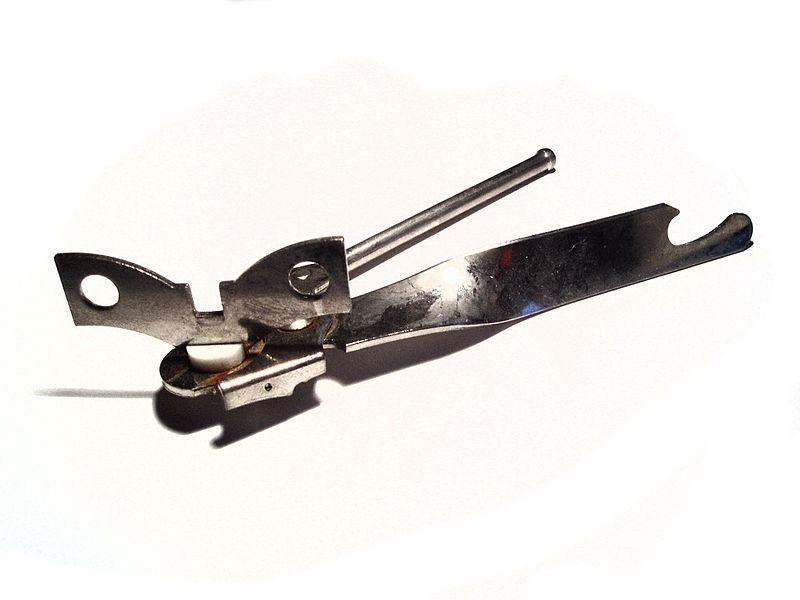
\includegraphics[width=0.3\textwidth]{pictures/800px-Can_Opener.jpg}
\label{fig:canOpener2}
\end{figure}

This version has a circular knife, which hides the sawing motion with a crank, but the pressure required to operate it makes it very clear that a knife is still cutting through metal.

\begin{figure}[H]
\centering
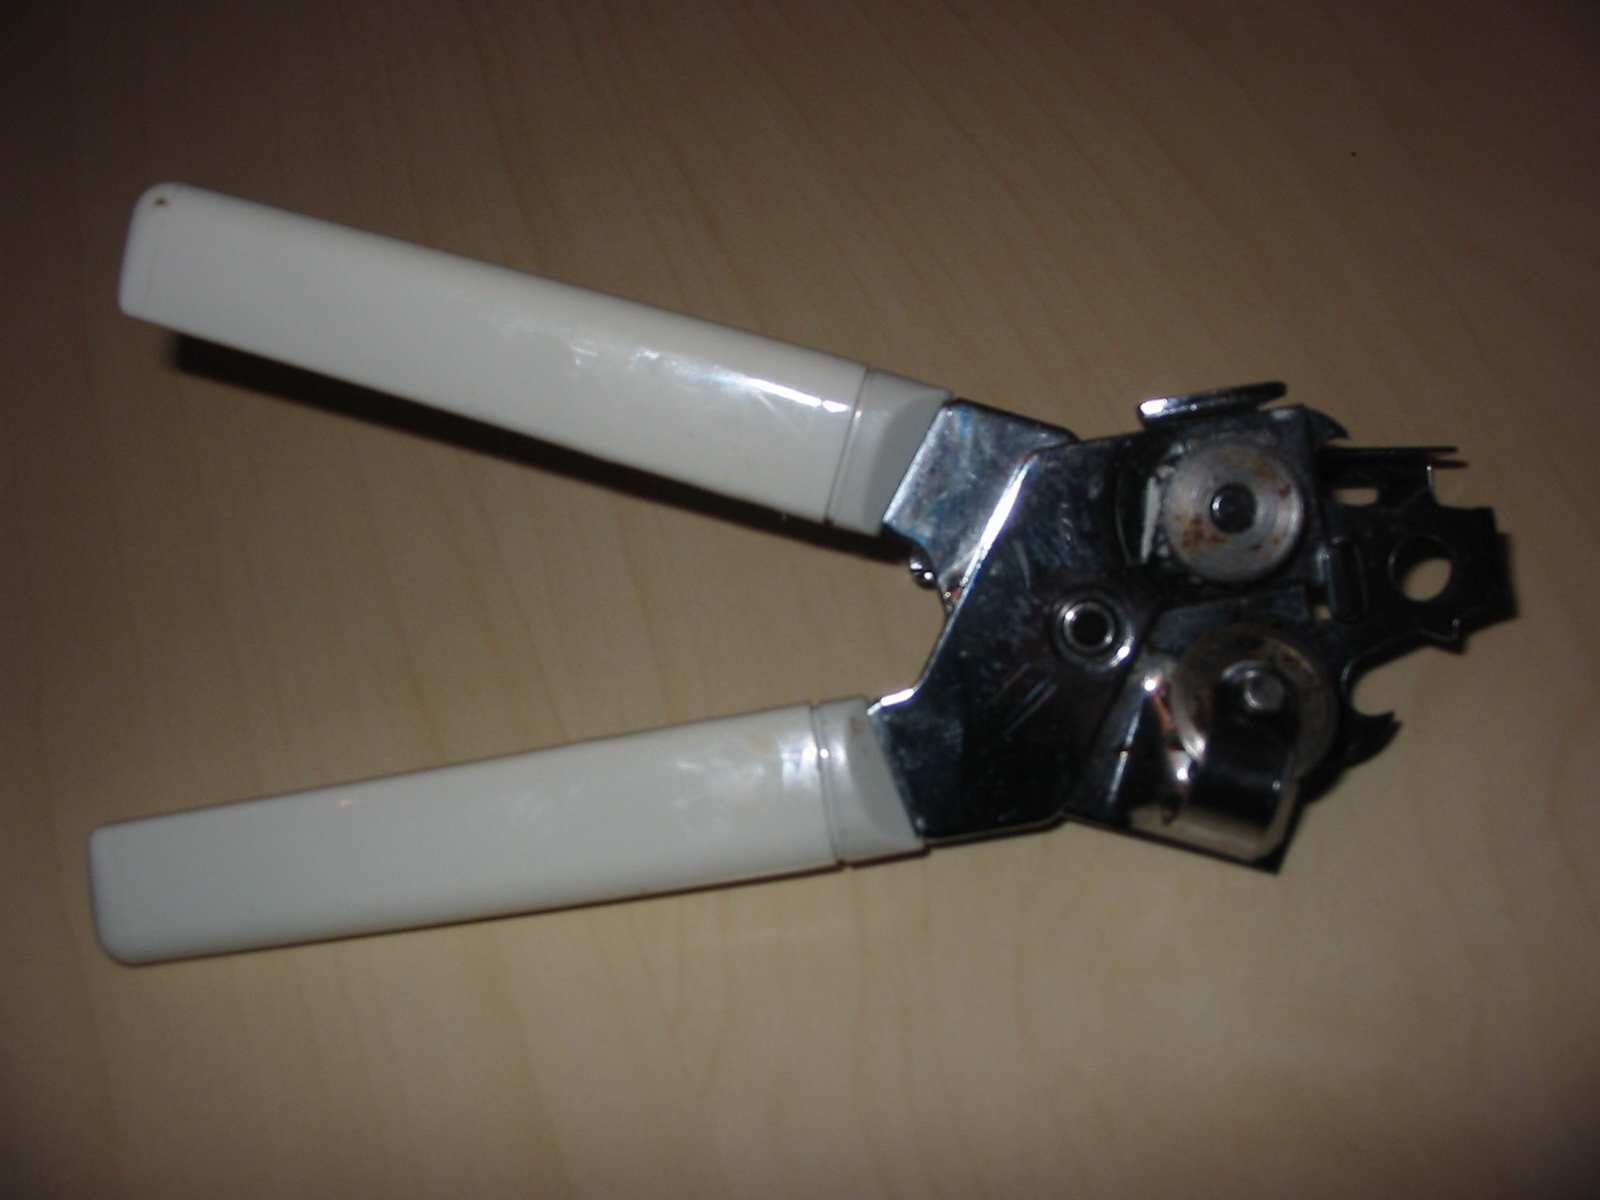
\includegraphics[width=0.3\textwidth]{pictures/Can_opener.JPG}
\label{fig:canOpener3}
\end{figure}

\subsection{Implementation}

An abstraction is really just a design until it is implemented in some way. It is possible to design an abstraction, and then have several different implementations, all with different strengths and weaknesses.

Suppose that you had been tasked to create a device to cook an egg without requiring the cook to crack the egg. One possible implementation for such an egg-cooking device is this

\begin{figure}[H]
\centering
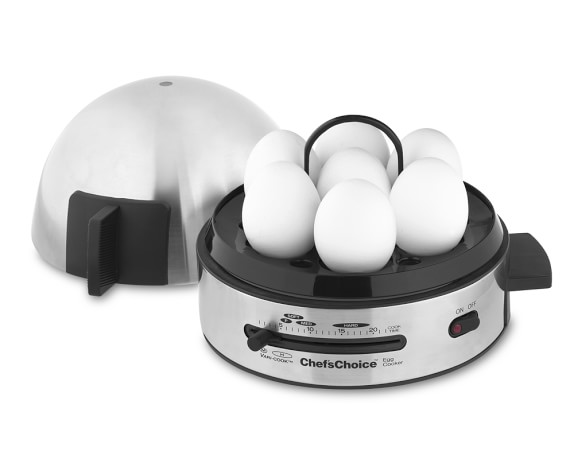
\includegraphics[width=0.3\textwidth]{pictures/chefschoice-electric-egg-cooker-c.jpg}
\label{fig:eggCooker1}
\end{figure}

Another possible implementation could look like this

\begin{figure}[H]
\centering
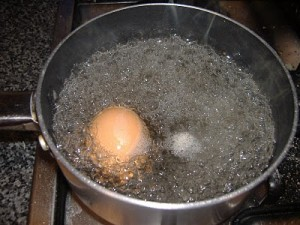
\includegraphics[width=0.3\textwidth]{pictures/boiled-egg-300x225.jpg}
\label{fig:eggCooker2}
\end{figure}


Another implementation can be found here:  \url{http://www.youtube.com/watch?v=XRb82E4_b38}

While these implementations accomplish the task, they are not equal in terms of cost to construct, maintainability, likelihood of breakdown, etc.



\section{Abstraction in Software Design}

The image below illustrates the different levels of abstraction required to create a computer program for managing a sports complex. The highest level of abstraction, the application level, maps the ideas and concepts of the real world to the specification of the program operation.

\begin{figure}[H]
\centering
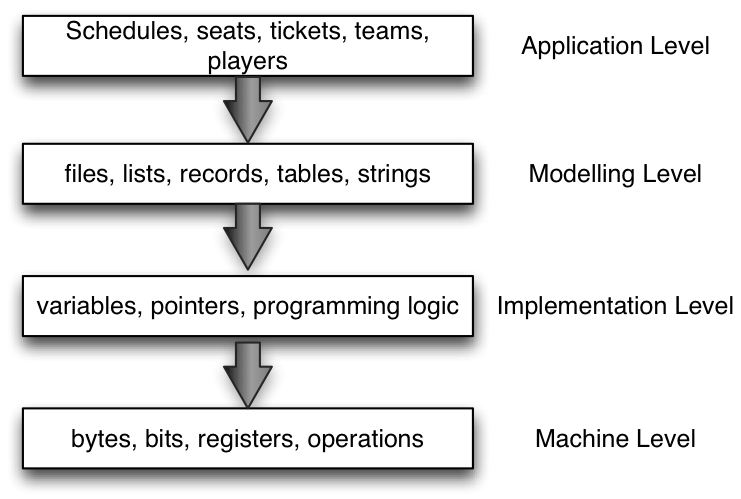
\includegraphics{pictures/abstraction01.png}
\label{fig:sportsComplex}
\end{figure}

The second level, the modeling level, maps the objects and entities discovered in the first level to models that can be used to represent the entities in the software. The third level of abstraction creates the actual implementation of those models and the last level is the responsibility of the compiler.

\textbf{In computing, an abstraction lets you understand 'what' can be accomplished without requiring that you know the details of 'how' the thing is accomplished.}

The reason we use abstractions in programming is really for economics. It is more time-efficient for programmers to reuse previously developed (and debugged) libraries than it is for them to program everything in binary. It is also more cost-efficient because the reusable library only needs to be debugged once, and then used many times. This is in contrast to building from scratch each time, which incurs the same debugging requirements for every development effort.

Programming languages, file system libraries, input-output libraries, and string libraries are all examples of abstractions that programmers use every day. Abstract data types 
are another kind of abstraction that programmers use.

Learning how to design a program in layers, and how to work at an appropriate level of abstraction for each layer is a crucial skill for software developers. Most developers are only concerned with the first three levels of abstraction (application, modeling, and implementation), and must learn how to design applications within those layers.

When you are writing software, you must first ensure that you understand the problem. Make sure you know what the software is supposed to do, and that you understand all the conditions surrounding its operation.

Your first task as a software developer is to decompose the problem into application-level constructs. Identify the main ideas in the software problem (like teams and schedules). These are the core 'things' that the software must create, but they are not things that the computer programming language knows anything about.

The second task is to identify a suitable model for each of the things you find in the first step. For example, you might decide that the best way to represent the teams is as a list, but that the best way to represent the ticket line is by using a queue.


In many cases, the developer can use third party libraries as the implementation layer for the models. Thoroughly debugged modules of abstract data types are available for nearly every programming language.
However, in this class you will be asked to create those modules . By the end of the course, you should have your own, thoroughly debugged, library of Abstract Data Types that you can reuse whenever you wish.

\subsection{Abstract Data Types}

Remember that specification (i.e. "what") and implementation (i.e. "how") are two separate things.
For example, if you are writing functions  in your code, the specification is the function header + pre/post conditions and the implementation is the local variables + body of subroutine.

When you are writing abstract data types, the specification is the definition of data type + operations defined on that type. The implementation is the program needed to effect those operations. In C the specification is usually a header file containing type and function declarations together with a .c file in which they are implemented.

Abstract data types are organized into modules. Each module contains the variable definitions (structures) and operations required to meet the specification of the ADT.

The module exports a 'type', such as list or tree or stack that a programmer can use to declare variables. The variables can then be manipulated using the operations defined within the ADT.

The most important part of this process is that the user of the variable types only needs to know WHAT is possible, but has no need to know HOW it is implemented. The type is abstract from the point of view of the user.

An abstract data type is usually provided to the developer in the form of a library or module.

Some operations are common to most ADT specifications. In particular, pretty much all ADT modules need to provide mechanisms for the following operations:
\begin{itemize}
\item Creating the ADT (initialization of internal variables/allocation of dynamic structures)
\item Destroying the ADT (management of de-allocation of dynamic resources)
\item Adding data to the ADT
\item Removing data from the ADT
\item Getting the value of data in the ADT
\end{itemize}
The details of how those operations behave vary in the different kinds of ADTs, but the core purpose of the operation remains constant.

\subsection{Worked Example: The Fraction ADT}

Suppose you were writing a program that required a representation of fractions. It is not always sufficient to convert  fractions to decimals, sometimes fractions need to stay as fractions. A fraction ADT that allowed the programmer to declare a variable of type fraction would be extremely useful.

First, we need a definition of what a fraction is. 
Fraction: A fraction is a number a/b where a,b are integers, b is non-zero.

\subsubsection{Operations}

The first step in designing an ADT is to imagine what operations are required. In addition to the core operations of create, insert, read, destroy the fraction ADT will need:

\begin{itemize}
\item add (subtraction is just adding with negative numbers)
\item multiply (really just repeated adding, but would be nice to have it as a separate operation)
\end{itemize}

\begin{lstlisting}
ADT specification for Fraction

create_fraction(numerator, denominator): Fraction
    preconditions: none
    postconditions: a fraction is created with the appropriate numerator 
                    and denominator
get_numerator(Fraction): number
    preconditions: an initialized Fraction is given as the parameter
    postconditions: none
get_denominator(Fraction): number
    preconditions: an initialized Fraction is given as the parameter
    postconditions: none
destroy_fraction(Fraction)
    preconditons: the parameter Fraction is initialized
    postconditions: the fraction is destroyed and memory released if necessary
add(Fraction, Fraction): Fraction
    preconditions: two initialized fractions are passed in as parameters
    postconditions: the two fractions are added together and the result is 
                    placed in a new Fraction variable that is returned to the 
                    calling procedure
\end{lstlisting}

The ADT could have many other operations as well.   For example, it could have a function to display/print a fraction or the ability to create a fraction  type from a string representation of the fraction (i.e. "one half" or "three fifths").

\subsubsection{Example Code}

Here's an example of what some of the fraction code might look like in C.  First, the .h file contains the definition of the struct as well as the prototypes for the functions that operate on that struct.

\begin{lstlisting}

/**
 * @file fraction.h
 * @author Judi McCuaig
 * @date January 2017
 * @brief API for a fraction ADT
 */
#ifndef _JRM_FRACTION
#define _JRM_FRACTION

fraction.h

typedef struct {
  int integer;
  int numerator;
  int denominator;
} Fraction;

/** Creates a fraction from an integer numerator and denominator
*@return NULL if the creation is unsuccessful
*@param integer value for the numerator
*@param integer value for the denominator
**/
Fraction * create_fraction(int numer, int denom);

/** Adds two fractions and returns a new fraction that is the result of the addition
*@return NULL if the addition is unsuccessful
*@param Pointer the first Fraction operand
*@param Pointer to the second Fraction operand
**/
Fraction * add ( Fraction *fractOne, Fraction *fractTwo );

#endif

\end{lstlisting}

The .c file doesn't need to redefine the struct because the .h file is included.  The .c file is used to flesh out the implementation of the functions.

\begin{lstlisting}
/**
 * @file fraction.c
 * @author Judi McCuaig
 * @date January 2017
 * @brief implementation of fraction ADT
 */
#include "fraction.h"

Fraction * create_fraction(int numer, int denom){
  Fraction * temp = malloc(sizeof(Fraction)*1);
  temp->numerator = numer;
  temp->denominator = denom;
  return(temp)
}

Fraction * add ( Fraction *fractOne, Fraction *fractTwo ){
  Fraction result= malloc(sizeof(Fraction)*1);
  int largeCommonDenominator;
  int part1, part2, numeratorResult;
  hcd = fractOne->denominator * fractTwo->denominator;
  part1 = fractTwo->denominator * fractOne->numerator;
  part2 = fractOne->denominator * fractTwo->numerator;
  numeratorResult = part1 + part2;
  result->numerator = numeratorResult;
  result->denominator = largeCommonDenominator;
  return result;
}
\end{lstlisting}

The fraction ADT can be used by simply including the .h file in the c program that needs the ADT and then compiling the fraction.c program in with the application.c program.

\begin{lstlisting}
/**
 * @file application.c
 * @author Judi McCuaig
 * @date January 2017
 * @brief use of Fraction ADT
 */
#include "fraction.h"

int main(void){
  Fraction * myFraction = create_fraction(1,2);
  Fraction * myOtherFraction = create_fraction(3,4);
  Fraction * theAnswer = add(myFraction, myOtherFraction);
}

\end{lstlisting}


\section{Information Hiding (Encapsulation)}
Information Hiding is one way to achieve abstraction.  The details of the library implementation are hidden by providing functions to perform operations on the data structure instead of allowing programmers to work directly with the attributes of the data structure. The user of the ADT must use ONLY the interface (the available operations) of the ADT and must resist the temptation to go 'under the hood' and use the component parts.

Information Hiding is also called encapsulation.  Encapsulation helps to prevent errors when a library of functions is updated. For example, suppose you were using a String ADT that provides a stringLength(String) operation to return the length of the string. Suppose further that you knew that the length of the string was stored as an integer in the ADT because you had looked at the source code.
If, in your code, you write int size = stringLength(myString); you are guaranteed (because of preconditions and postconditions) that you will get the length of the string returned.

However, if you  chose to ignore the encapsulation and bypassed the interface, writing the following instead int size = myString->length you could end up with code that gave errors.  In this situation what would happen if the author of the String library gives you an update that changes the declaration of length in the struct from int to double? Your previously working code will break, because you didn't use the interface.


\section{Extending Activities}

\begin{itemize}

\item  Compile a list of 10 different programming languages. Categorize the languages on your list based on their level of abstraction (Moderate, High, Very High).

\item  {\textbf{Sidequest: Rube-Goldberg Machines}

Another example of implementation differences can be found in the notion of Rub-Goldberg machines. A Rube-Goldberg machine is something that performs a simple task in as complex a way as possible.
There are several examples of Rube Goldberg machines for making toast on YouTube. Find at least three, watch the video, and count the number of steps in each machine.
As you can see, even though the task specified for a Rube Goldberg machine is simple, the implementations of that specification are endless.
For a silly example of a Rube-Goldberg machine, have a look at: \url{http://www.youtube.com/watch?v=lCYg_gz4fDo}
The point of this diversion is that it is really easy, especially in software construction, to meet the specifications for a program, but to do it with the software equivalent of a rube-goldberg machine and end up with something that works, but is not easily understood and is difficult to maintain.}

\item  Write pseudocode for a multiply and a subtract operation for the fraction ADT
What does the integer portion of the Fraction struct represent? List any additional operation(s) would be required in order to make use of that part of the struct.

 \end{itemize}